\documentclass[openany]{book}

\input{../../../latex_preambule_style/preambule}
\input{../../../latex_preambule_style/styleCoursCycle4}
\input{../../../latex_preambule_style/styleExercices}
\input{../../../latex_preambule_style/styleExercicesAideCompetences}
%\input{../../latex_preambule_style/styleCahier}
\input{../../../latex_preambule_style/bas_de_page_cycle4}
\input{../../../latex_preambule_style/algobox}


%%%%%%%%%%%%%%%  Affichage ou impression  %%%%%%%%%%%%%%%%%%
\newcommand{\impress}[2]{
\ifthenelse{\equal{#1}{1}}  %   1 imprime / affiche sur livre  -----    0 affiche sur cahier 
{%condition vraieé
#2
}% fin condition vraie
{%condition fausse
}% fin condition fausse
} % fin de la procédure
%%%%%%%%%%%%%%%  Affichage ou impression  %%%%%%%%%%%%%%%%%%
 \usepackage{geometry}
 \geometry{top=1.5cm, bottom=0cm, left=2cm , right=2cm}
%%%%%%%%%%%%%%%%%%%%%%%%%%%%%%%%%%%%%%%%%%%%%%%%

\begin{document}


\begin{seance}[Statistiques]

\begin{description}
\item[$\square$]  Calculer et interpréter des caractéristiques de position ou de dispersion d’une série statistique - Indicateurs : moyenne, médiane, étendue.
\item[$\square$] Calculer des effectifs, des fréquences.
\item[$\square$] Lire des données sous forme de données brutes, de tableau, de graphique.
\end{description}
\end{seance}


\Exe


Voici les notes obtenues tout au long de l'année par un élève de 4\ieme\ en
mathématiques (toutes les notes sont sur 20) :\\
\begin{tabular}{|*{3}{p{3.5cm}|}}
\hline
\bf Trimestre 1 & \bf Trimestre 2 & \bf Trimestre 3 \\ \hline
12 -- 15 -- 7 -- 10 & 10 -- 12 -- 14 & 17 -- 11 -- 9 -- 14 -- 14 \\
\hline
\end{tabular}
\begin{enumerate}
\item Calculer la moyenne pour chaque trimestre. Calculer alors la moyenne
	annuelle. 
\item Calculer la moyenne de l'ensemble des notes obtenues tout au long
	de l'année. Quelle remarque peut-on faire ? Commenter.
	
\end{enumerate}

\Exe


Pierre, Jean et Alain ont passé un examen comportant quatre
disciplines. Pour être reçu, il faut atteindre 10 de moyenne.
\begin{enumerate}
\item Calculer la moyenne, sans coefficient, des trois candidats.
\begin{center}
  \begin{tabular}{|c|c|c|c|c|}
\cline{2-5}
\multicolumn{1}{c|}{}&Français&Mathématiques&Anglais&Technologie\\
\hline
Pierre&15&9&11&7\\
\hline
Jean&10&11&12&9\\
\hline
Alain&7&14&13&8\\
\hline
  \end{tabular}
\end{center}
\item Pour cet examen, le français, les mathématiques, l'anglais et la
technologie ont respectivement pour coefficient 6; 4; 2 et 5.\par
Calculer la moyenne pondérée de chaque candidat et dire s'ils sont reçus
ou non.
\end{enumerate}

\Exe


\begin{multicols}{2}
Voici ci-contre la répartition par âge des membres d'un club d'échec.
Quel est l'age moyen des adhérents ?

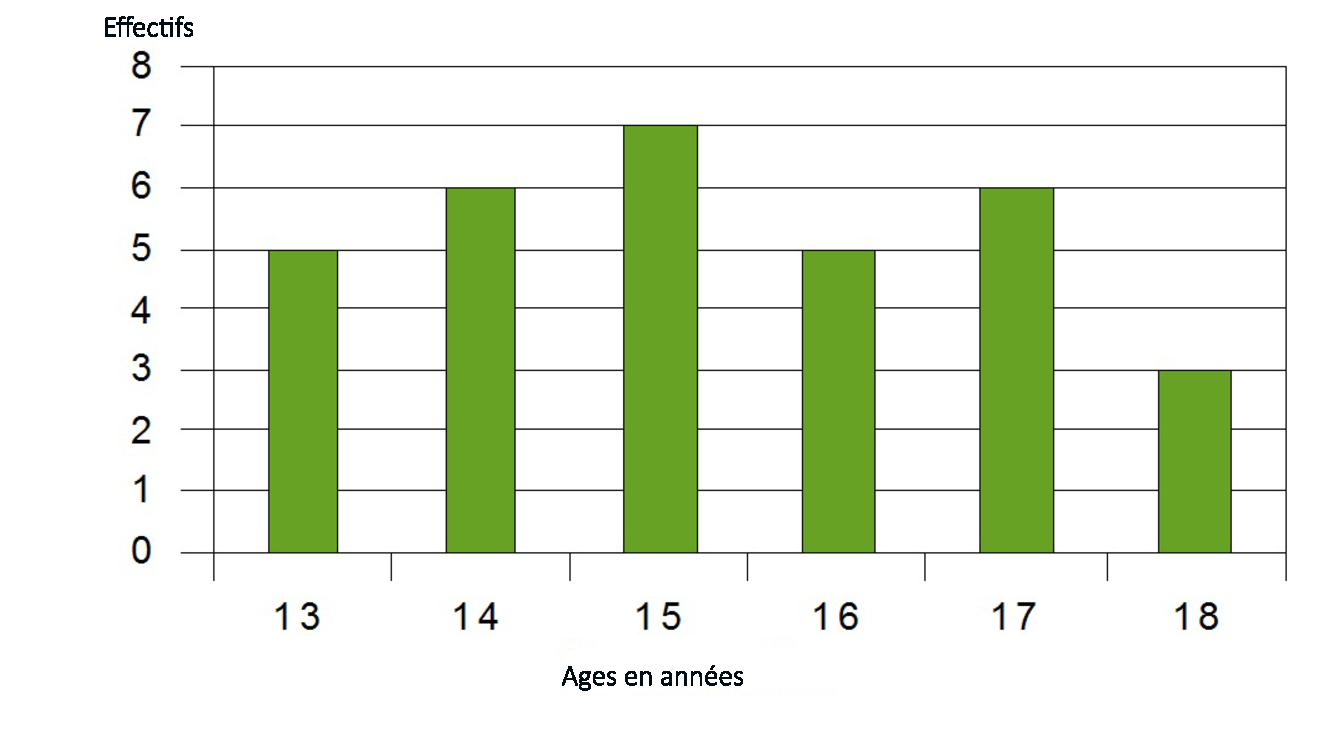
\includegraphics[scale=0.35]{Stat-cours1.eps} 
\end{multicols}	


\begin{seance}[Statistiques]

\begin{description}
\item[$\square$]  Calculer et interpréter des caractéristiques de position ou de dispersion d’une série statistique - Indicateurs : moyenne, médiane, étendue.
\item[$\square$] Calculer des effectifs, des fréquences.
\item[$\square$] Lire des données sous forme de données brutes, de tableau, de graphique.
\end{description}
\end{seance}

\Exe


\begin{minipage}{0.5\linewidth}
Le graphique ci-dessous montre les résultats à un contrôle de sciences obtenus par deux groupes d'élèves, désignés par « Groupe A » et « Groupe B ». 
La note moyenne pour le Groupe A est de 62,0 et de 64,5 pour le Groupe B. Les élèves réussissent ce contrôle lorsque leur note est de 50 points ou davantage. Sur la base de ce graphique, le professeur conclut que le Groupe B a mieux réussi ce contrôle que le Groupe A. Les élèves du Groupe A ne sont pas d'accord avec le professeur. Ils essaient de le convaincre que le Groupe B n'a pas nécessairement mieux réussi. \hfill{{\scriptsize D'après PISA 2009}}
\end{minipage}
\begin{minipage}{0.5\linewidth}
\begin{center}
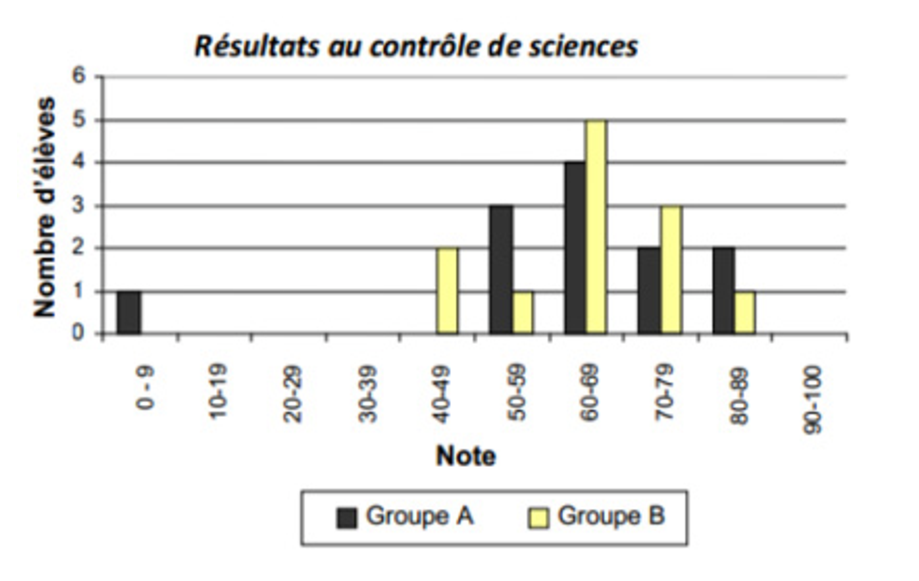
\includegraphics[scale=0.6]{Stat-13.eps} 
\end{center}
\end{minipage}
En vous servant du graphique, donnez un argument mathématique que les élèves du Groupe A pourraient utiliser. 




\Exe


On a représenté sur le diagramme suivant les vols du mois de février d’une compagnie aérienne.  
\begin{center}
\definecolor{xdxdff}{rgb}{0.49019607843137253,0.49019607843137253,1.}
\definecolor{ffdxqq}{rgb}{1.,0.8431372549019608,0.}
\definecolor{ffffqq}{rgb}{1.,1.,0.}
\definecolor{ffxfqq}{rgb}{1.,0.4980392156862745,0.}
\definecolor{ffqqqq}{rgb}{1.,0.,0.}
\definecolor{xfqqff}{rgb}{0.4980392156862745,0.,1.}
\definecolor{qqqqff}{rgb}{0.,0.,1.}
\begin{tikzpicture}[line cap=round,line join=round,>=triangle 45,x=1.0cm,y=1.0cm]
\clip(-0.096,-0.204) rectangle (18.304,8.336);
\draw[color=xfqqff,fill=xfqqff,fill opacity=1.0] (5.,3.5757359312880714) -- (5.424264068711929,3.5757359312880714) -- (5.424264068711929,4.) -- (5.,4.) -- cycle; 
\draw [shift={(5.,4.)},color=ffqqqq,fill=ffqqqq,fill opacity=1.0] (0,0) -- (0.:0.6) arc (0.:30.488940499830935:0.6) -- cycle;
\draw [shift={(5.,4.)},color=ffxfqq,fill=ffxfqq,fill opacity=0.95] (0,0) -- (30.488940499830935:0.6) arc (30.488940499830935:59.44286434307001:0.6) -- cycle;
\draw [shift={(5.,4.)},fill=black,fill opacity=1.0] (0,0) -- (59.44286434307001:0.6) arc (59.44286434307001:90.:0.6) -- cycle;
\draw [shift={(5.,4.)},color=qqqqff,fill=qqqqff,fill opacity=0.44]  plot[domain=1.5707963267948966:4.71238898038469,variable=\t]({1.*4.*cos(\t r)+0.*4.*sin(\t r)},{0.*4.*cos(\t r)+1.*4.*sin(\t r)});
\draw [shift={(5.,4.)},color=xfqqff,fill=xfqqff,fill opacity=0.66]  (0,0) --  plot[domain=-1.5707963267948966:0.,variable=\t]({1.*4.*cos(\t r)+0.*4.*sin(\t r)},{0.*4.*cos(\t r)+1.*4.*sin(\t r)}) -- cycle ;
\draw [shift={(5.,4.)},color=ffqqqq,fill=ffqqqq,fill opacity=0.6]  (0,0) --  plot[domain=0.:0.5321323971666955,variable=\t]({1.*4.*cos(\t r)+0.*4.*sin(\t r)},{0.*4.*cos(\t r)+1.*4.*sin(\t r)}) -- cycle ;
\draw [shift={(5.,4.)},color=ffxfqq,fill=ffxfqq,fill opacity=0.4]  (0,0) --  plot[domain=0.5321323971666955:1.037473699602908,variable=\t]({1.*3.973415659102379*cos(\t r)+0.*3.973415659102379*sin(\t r)},{0.*3.973415659102379*cos(\t r)+1.*3.973415659102379*sin(\t r)}) -- cycle ;
\draw [shift={(5.,4.)},color=ffffqq,fill=ffffqq,fill opacity=0.5]  (0,0) --  plot[domain=1.037473699602908:1.5707963267948966,variable=\t]({1.*4.*cos(\t r)+0.*4.*sin(\t r)},{0.*4.*cos(\t r)+1.*4.*sin(\t r)}) -- cycle ;
\draw (10.644,6.776) node[anchor=north west] {Vols vers l'Asie};
\draw (10.664,6.176) node[anchor=north west] {Vols vers l'Afrique};
\draw (10.664,5.616) node[anchor=north west] {Vols vers l'Amérique};
\draw (10.704,5.056) node[anchor=north west] {Vols vers l'Europe};
\draw (10.724,4.436) node[anchor=north west] {Vols vers la France};
\begin{scriptsize}
\draw [fill=ffffqq] (10.304,6.636) circle (2.5pt);
\draw [fill=ffdxqq] (10.304,6.036) circle (2.5pt);
\draw [fill=ffqqqq] (10.324,5.436) circle (2.5pt);
\draw [fill=xfqqff] (10.344,4.836) circle (2.5pt);
\draw [fill=xdxdff] (10.364,4.236) circle (2.5pt);
\end{scriptsize}
\end{tikzpicture}
\end{center}

\begin{minipage}{8cm}
Dans chaque cas, quelle fréquence représentent les vols vers la France, l’Europe et l’Asie. 
\end{minipage}
\begin{minipage}{1cm}
$~~$
\end{minipage}
\begin{minipage}{8cm}
Au mois de février, cette compagnie a affrété 576 vols. Calculer le nombre de vols vers la France, l’Europe et l’Asie. 
\end{minipage}


\Exe


Si 2/5 des habitants d'un pays ont au moins 50 ans et 1/3 des habitants de ce pays ont moins de 20 ans, est-il possible que l'âge moyen de la population soit de 40 ans ?

\hfill{D’après le cadre d’évaluation «PISA 2006»:}
 
\hfill{items libérés Mathématiques OCDE/DEPP – janvier 2011}

 





\begin{seance}[Statistiques]

\begin{description}
\item[$\square$]  Calculer et interpréter des caractéristiques de position ou de dispersion d’une série statistique - Indicateurs : moyenne, médiane, étendue.
\item[$\square$] Calculer des effectifs, des fréquences.
\item[$\square$] Lire des données sous forme de données brutes, de tableau, de graphique.
\end{description}
\end{seance}




\Dnb

Une entreprise de fabrication de bonbons souhaite vérifier la qualité de sa nouvelle
machine de conditionnement. Cette machine est configurée pour emballer environ $60$
bonbons par paquet. Pour vérifier sa bonne configuration, on a étudié $500$~paquets à
la sortie de cette machine.

\medskip

\textbf{Document 1 : Résultats de l'étude}

\begin{center}
\begin{tabularx}{\linewidth}{|m{2cm}|*{9}{>{\centering \arraybackslash}X|}}\hline
Nombre de bonbons	&56 &57 &58 &59 &60 	&61 &62 &63 &64\\ \hline
Effectifs 			&4 	&36 &53 &79 &145 	&82 &56 &38 &7\\ \hline
\end{tabularx}
\end{center}

\textbf{Document 2 : Critères de qualité}

\medskip

Pour être validée par l'entreprise, la machine doit respecter trois critères de qualité:

\setlength\parindent{8mm}
\begin{itemize}
\item[$\bullet~~$] Le nombre moyen de bonbons dans un paquet doit être compris entre 59,9 et
60,1.
\item[$\bullet~~$] L'étendue de la série doit être inférieure ou égale à $10$.
\item[$\bullet~~$] La médiane doit être comprise entre 59 et 61.
\end{itemize}
\setlength\parindent{0mm} 
 
La nouvelle machine respecte-t-elle les critères de qualité ?
 
\emph{Il est rappelé que les réponses doivent être justifiées.}

\Dnb

On lance deux dés tétraédriques, équilibrés et non truqués, dont les faces sont
numérotées de 1 à 4. On calcule la somme des nombres lus sur chacune des faces sur
lesquelles reposent les dés.

\smallskip

\np{1000} lancers sont simulés avec un tableur. Le graphique suivant représente la
fréquence d'apparition de chaque somme obtenue :

\begin{center}
\psset{xunit=1cm,yunit=0.2cm}
\begin{pspicture}(-1,-5)(9,25)
\psaxes[linewidth=1.25pt,Dx=10,Dy=5](0,0)(9,25)
\multido{\n=1+1}{8}{\uput[d](\n,0){\n}}
\psframe[fillstyle=solid,fillcolor=lightgray](1.5,0)(2.5,7)
\psframe[fillstyle=solid,fillcolor=lightgray](2.5,0)(3.5,15)
\psframe[fillstyle=solid,fillcolor=lightgray](3.5,0)(4.5,19)
\psframe[fillstyle=solid,fillcolor=lightgray](4.5,0)(5.5,23)
\psframe[fillstyle=solid,fillcolor=lightgray](5.5,0)(6.5,17)
\psframe[fillstyle=solid,fillcolor=lightgray](6.5,0)(7.5,13)
\psframe[fillstyle=solid,fillcolor=lightgray](7.5,0)(8.5,6)
\rput(4.5,-4){somme des nombres inscrits sur les deux dés} \rput{90}(-1,12.5){fréquence en \,\%}
\end{pspicture}
\end{center}

\begin{enumerate}
\item Par lecture graphique donner la fréquence d'apparition de la somme 3.
\item Lire la fréquence d'apparition de la somme 1 ? Justifier cette fréquence.
\item  
	\begin{enumerate}
		\item Décrire les lancers de dés qui permettent d'obtenir une somme égale à 3.
		\item En déduire la probabilité d'obtenir la somme 3 en lançant les dés. On exprimera
cette probabilité en pourcentage. Expliquer pourquoi ce résultat est différent de celui obtenu à la question 1.
	\end{enumerate} 
 \end{enumerate}


\begin{seance}[Statistiques]

\begin{description}
\item[$\square$]  Calculer et interpréter des caractéristiques de position ou de dispersion d’une série statistique - Indicateurs : moyenne, médiane, étendue.
\item[$\square$] Calculer des effectifs, des fréquences.
\item[$\square$] Lire des données sous forme de données brutes, de tableau, de graphique.
\end{description}
\end{seance}

\Dnb

Une association cycliste organise une journée de randonnée à  vélo.

Les participants ont le choix entre trois circuits de longueurs différentes: 42 km, 35 km et 27 km.

À l'arrivée, les organisateurs relèvent les temps de parcours des participants et calculent leurs vitesses moyennes. Ils regroupent les informations dans un tableau dont voici un extrait:

\begin{center}
\begin{tabularx}{\linewidth}{|l|*{5}{>{\centering \arraybackslash}X|}}\hline
Nom du sportif				& Alix 	&David 	&Gwenn 		&Yassin 	&Zoé\\ \hline
Distance parcourue (en km)	& 35 	&42 	&27 		&35 		&42\\ \hline
Durée de la randonnée 		&2 h 	&3 h 	&1 h 30 min &1 h 45 min &1 h 36 min\\ \hline
Vitesse moyenne (en km/h) 	&17,5	&		&			&			&\\ \hline
\end{tabularx}
\end{center}


\begin{enumerate}
\item Quelle distance David a-t-il parcourue ?
\item Calculer les vitesses moyennes de David et de Gwenn.
\item Afin d'automatiser les calculs, l'un des organisateurs décide d'utiliser la feuille de tableur ci-dessous :

\begin{center}
\begin{tabularx}{\linewidth}{|c|l|*{5}{>{\centering \arraybackslash}X|}}\hline
&A &B &C &D& E &F\\ \hline
1 &Nom du sportif 				&Alix 	&David 	&\footnotesize Gwenn 	&Yassin &Zoé\\ \hline
2 &Distance parcourue (en km)	& 35	& 42	&27 	&35 	&42\\ \hline
3 &Durée de la randonnée (en h)	& 2 	&3 		&1,5	&		&\\ \hline
4 &Vitesse moyenne (en km/h)	& 17,5	&		&		&		&\\ \hline
\end{tabularx}
\end{center}

	\begin{enumerate}
		\item Quel nombre doit-il saisir dans la cellule E3 pour renseigner le temps de Yassin ?
		\item Expliquer pourquoi il doit saisir 1,6 dans la cellule F3 pour renseigner le temps de Zoé.
		\item Quelle formule de tableur peut-il saisir dans la cellule B4 avant de l'étirer sur la ligne 4 ?
	\end{enumerate}
\item Les organisateurs ont oublié de noter la performance de Stefan.
	
Sa montre GPS indique qu'il a fait le circuit de 35 km à  la vitesse moyenne de 25 km/h.
	
Combien de temps a-t-il mis pour faire sa randonnée? On exprimera la durée de la randonnée en
heures et minutes.
\end{enumerate}



\begin{seance}[Statistiques]

\begin{description}
\item[$\square$]  Calculer et interpréter des caractéristiques de position ou de dispersion d’une série statistique - Indicateurs : moyenne, médiane, étendue.
\item[$\square$] Calculer des effectifs, des fréquences.
\item[$\square$] Lire des données sous forme de données brutes, de tableau, de graphique.
\end{description}
\end{seance}


\Dnb

Une coopérative collecte le lait dans différentes exploitations agricoles.

Le détail, de la collecte du jour ont été saisis dans une feuille de calcul d'un tableur.

\begin{center}
\begin{tabularx}{0.7\linewidth}{|c|*{2}{>{\centering \arraybackslash}X|}}\hline
&A&B \\ \hline
1&Exploitation agricole& Quantité de lait collecté (en L)\\ \hline
2& Beausejour& \np{1250}\\ \hline
3&Le Verger& \np{2130}\\ \hline 
4&La  Fourragère& \np{1070}\\ \hline
5& Petit pas& \np{2260}\\ \hline
6&La  Chausse Pierre& \np{1600}\\ \hline
7& Le Palet& \np{1740}\\ \hline
8&Quantité totale de lait collecté&\\ \hline
\end{tabularx}
\end{center}

\begin{enumerate}
\item Une formule doit être saisie dans la cellule B8 pour obtenir la quantité totale de lait collecté. Parmi les quatre propositions ci-dessous, recopier celle qui convient.

\begin{center}
\begin{tabularx}{\linewidth}{|*{4}{>{\centering \arraybackslash}X|}}\hline
SOMME(B2~:~B7)&SOMME(B2~:~B8)&=SOMME(B2~:~B7)&=SOMME(B2~:~B8)\\ \hline
\end{tabularx}
\end{center}
\medskip
\item  
\begin{enumerate}
\item  \textit{Calculer la différence entre la quantités de lait collecté la plus importante et celle la moins importante.}
\item \textit{Que représente pour la série statistique cette différence ?}
\end{enumerate}
\item  Calculer la moyenne des quantités de lait collecté dans ces exploitations.
\item  \textit{Calculer la médiane des quantités de lait collecté dans ces exploitations.}
\item  Quel pourcentage de la collecte provient de l'exploitation \og Petit Pas \fg{} ? On arrondira le résultat à l'unité.
\end{enumerate}



\end{document}